\chapter{Задача о распределении ресурсов} 
Имеется однородный ресурс в количестве S = 6 единиц, который должен быть распределен между N = 6 предприятиями.\\
Использование i-м предприятием $x_{i}$ единиц ресурса дает доход, определяемый значением нелинейной функции $f_{i}(x_{i})$ (см. таблицу). Требуется найти распределение ресурсов между предприятиями, обеспечивающее максимальный доход.

\begin{center}
    \begin{tabular}{|a | c | c | c | c | c | c|} 
        \hline
             & \multicolumn{6}{c|}{предприятия}\\
         \hline
         \rowcolor{LightGray}
            & 1 & 2 & 3 & 4 & 5 & 6\\
        \hline
            0 & 0 & 0 & 0 & 0 & 0 & 0 \\
         \hline
            1 & 3 & 1 & 2 & 4 & 6 & 5 \\
         \hline
            2 & 4 & 5 & 8 & 1 & 4 & 4 \\
         \hline
            3 & 6 & 4 & 3 & 7 & 7 & 3 \\
         \hline
            4 & 2 & 7 & 1 & 2 & 3 & 2 \\
        \hline
            5 & 5 & 3 & 5 & 9 & 5 & 1 \\
         \hline
            6 & 6 & 1 & 7 & 4 & 2 & 4 \\
         \hline
    \end{tabular}
\end{center}

\begin{center}
    {\bf
    Решение:}
\end{center}

\begin{center}
    $F = \displaystyle \sum_{i=1}^{6} f_{i}(x_{i}) \rightarrow max$\\
    $\displaystyle \sum_{i=1}^{6} x_{i} = 6, x_{i} \ge 0, i = \overline{1, 6}$
\end{center}

\subsection*{1)} Оценим эффективность выделения ресурса на 1-е предприятие:\\
$\varphi_1(x) = \stackrel[0 \le x_1 \le x]{}{max}  \{f_1(x_1)\}$\\
$\varphi_1(0) = 0, x_1^0 = 0$\\
$\varphi_1(1) = max\{0; 3\} = 3, x_1^0 = 1$\\
$\varphi_1(2) = max\{0; 3; 4\} = 4, x_1^0 = 2$\\
$\varphi_1(3) = max\{0; 3; 4; 6\} = 6, x_1^0 = 3$\\
$\varphi_1(4) = max\{0; 3; 4; 6; 2\} = 6, x_1^0 = 3$\\
$\varphi_1(5) = max\{0; 3; 4; 6; 2; 5\} = 6, x_1^0 = 3$\\
$\varphi_1(6) = max\{0; 3; 4; 6; 2; 5; 6\} = 6, x_1^0 = 3$\\

\subsection*{2)} Оценим эффективность выделения ресурса на 1-е, 2-е предприятия:\\
$\varphi_2(x) = \stackrel[0 \le x_2 \le x]{}{max}  \{f_2(x_2) + \varphi_1(x - x_2)\}$\\

$\varphi_2(0) = 0, x_2^0 = 0$\\

$\varphi_2(1) = max \begin{Bmatrix}
    f_2(0) + \varphi_1(1 - 0) \\
    f_2(1) + \varphi_1(1 - 1) \\
\end{Bmatrix} = max \begin{Bmatrix}
    0 + 3 \\
    1 + 0 \\
\end{Bmatrix} = 3, x_2^0 = 0$\\

$\varphi_2(2) = max \begin{Bmatrix}
    f_2(0) + \varphi_1(2 - 0) \\
    f_2(1) + \varphi_1(2 - 1) \\
    f_2(2) + \varphi_1(2 - 2) \\
\end{Bmatrix} = max \begin{Bmatrix}
    0 + 4 \\
    1 + 3 \\
    5 + 0 \\
\end{Bmatrix} = 5, x_2^0 = 2$\\

$\varphi_2(3) = max \begin{Bmatrix}
    f_2(0) + \varphi_1(3 - 0) \\
    f_2(1) + \varphi_1(3 - 1) \\
    f_2(2) + \varphi_1(3 - 2) \\
    f_2(3) + \varphi_1(3 - 3) \\
\end{Bmatrix} = max \begin{Bmatrix}
    0 + 6 \\
    1 + 4 \\
    5 + 3 \\
    4 + 0 \\
\end{Bmatrix} = 8, x_2^0 = 2$\\

$\varphi_2(4) = max \begin{Bmatrix}
    f_2(0) + \varphi_1(4 - 0) \\
    f_2(1) + \varphi_1(4 - 1) \\
    f_2(2) + \varphi_1(4 - 2) \\
    f_2(3) + \varphi_1(4 - 3) \\
    f_2(4) + \varphi_1(4 - 4) \\
\end{Bmatrix} = max \begin{Bmatrix}
    0 + 6 \\
    1 + 6 \\
    5 + 4 \\
    4 + 3 \\
    7 + 0 \\
\end{Bmatrix} = 9, x_2^0 = 2$\\

$\varphi_2(5) = max \begin{Bmatrix}
    f_2(0) + \varphi_1(5 - 0) \\
    f_2(1) + \varphi_1(5 - 1) \\
    f_2(2) + \varphi_1(5 - 2) \\
    f_2(3) + \varphi_1(5 - 3) \\
    f_2(4) + \varphi_1(5 - 4) \\
    f_2(5) + \varphi_1(5 - 5) \\
\end{Bmatrix} = max \begin{Bmatrix}
    0 + 6 \\
    1 + 6 \\
    5 + 6 \\
    4 + 4 \\
    7 + 3 \\
    3 + 0 \\
\end{Bmatrix} = 11, x_2^0 = 2$\\

$\varphi_2(6) = max \begin{Bmatrix}
    f_2(0) + \varphi_1(6 - 0) \\
    f_2(1) + \varphi_1(6 - 1) \\
    f_2(2) + \varphi_1(6 - 2) \\
    f_2(3) + \varphi_1(6 - 3) \\
    f_2(4) + \varphi_1(6 - 4) \\
    f_2(5) + \varphi_1(6 - 5) \\
    f_2(6) + \varphi_1(6 - 6) \\
\end{Bmatrix} = max \begin{Bmatrix}
    0 + 6 \\
    1 + 6 \\
    5 + 6 \\
    4 + 6 \\
    7 + 4 \\
    3 + 3 \\
    1 + 0 \\
\end{Bmatrix} = 11, x_2^0 = 2$\\


\subsection*{3)} Оценим эффективность выделения ресурса на 1-е, 2-е, 3-е предприятия:\\
$\varphi_3(x) = \stackrel[0 \le x_3 \le x]{}{max}  \{f_3(x_3) + \varphi_2(x - x_3)\}$\\

$\varphi_3(0) = 0, x_3^0 = 0$\\

$\varphi_3(1) = max \begin{Bmatrix}
    f_3(0) + \varphi_2(1 - 0) \\
    f_3(1) + \varphi_2(1 - 1) \\
\end{Bmatrix} = max \begin{Bmatrix}
    0 + 3 \\
    2 + 0 \\
\end{Bmatrix} = 3, x_3^0 = 0$\\

$\varphi_3(2) = max \begin{Bmatrix}
    f_3(0) + \varphi_2(2 - 0) \\
    f_3(1) + \varphi_2(2 - 1) \\
    f_3(2) + \varphi_2(2 - 2) \\
\end{Bmatrix} = max \begin{Bmatrix}
    0 + 5 \\
    2 + 3 \\
    8 + 0 \\
\end{Bmatrix} = 5, x_3^0 = 0$\\

$\varphi_3(3) = max \begin{Bmatrix}
    f_3(0) + \varphi_2(3 - 0) \\
    f_3(1) + \varphi_2(3 - 1) \\
    f_3(2) + \varphi_2(3 - 2) \\
    f_3(3) + \varphi_2(3 - 3) \\
\end{Bmatrix} = max \begin{Bmatrix}
    0 + 8 \\
    2 + 5 \\
    8 + 3 \\
    3 + 0 \\
\end{Bmatrix} = 11, x_3^0 = 2$\\

$\varphi_3(4) = max \begin{Bmatrix}
    f_3(0) + \varphi_2(4 - 0) \\
    f_3(1) + \varphi_2(4 - 1) \\
    f_3(2) + \varphi_2(4 - 2) \\
    f_3(3) + \varphi_2(4 - 3) \\
    f_3(4) + \varphi_2(4 - 4) \\
\end{Bmatrix} = max \begin{Bmatrix}
    0 + 9 \\
    2 + 8 \\
    8 + 5 \\
    3 + 3 \\
    1 + 0 \\
\end{Bmatrix} = 13, x_3^0 = 2$\\

$\varphi_3(5) = max \begin{Bmatrix}
    f_3(0) + \varphi_2(5 - 0) \\
    f_3(1) + \varphi_2(5 - 1) \\
    f_3(2) + \varphi_2(5 - 2) \\
    f_3(3) + \varphi_2(5 - 3) \\
    f_3(4) + \varphi_2(5 - 4) \\
    f_3(5) + \varphi_2(5 - 5) \\
\end{Bmatrix} = max \begin{Bmatrix}
    0 + 11 \\
    2 + 9 \\
    8 + 8 \\
    3 + 5 \\
    1 + 3 \\
    5 + 0 \\
\end{Bmatrix} = 16, x_3^0 = 2$\\

$\varphi_3(6) = max \begin{Bmatrix}
    f_3(0) + \varphi_2(6 - 0) \\
    f_3(1) + \varphi_2(6 - 1) \\
    f_3(2) + \varphi_2(6 - 2) \\
    f_3(3) + \varphi_2(6 - 3) \\
    f_3(4) + \varphi_2(6 - 4) \\
    f_3(5) + \varphi_2(6 - 5) \\
    f_3(6) + \varphi_2(6 - 6) \\
\end{Bmatrix} = max \begin{Bmatrix}
    0 + 11 \\
    2 + 11 \\
    8 + 9 \\
    3 + 8 \\
    1 + 5 \\
    5 + 3 \\
    7 + 0 \\
\end{Bmatrix} = 17, x_3^0 = 2$\\


\subsection*{4)} Оценим эффективность выделения ресурса на 1-е, 2-е, 3-е, 4-е предприятия:\\
$\varphi_4(x) = \stackrel[0 \le x_4 \le x]{}{max}  \{f_4(x_4) + \varphi_3(x - x_4)\}$\\

$\varphi_4(0) = 0, x_4^0 = 0$\\

$\varphi_4(1) = max \begin{Bmatrix}
    f_4(0) + \varphi_3(1 - 0) \\
    f_4(1) + \varphi_3(1 - 1) \\
\end{Bmatrix} = max \begin{Bmatrix}
    0 + 3 \\
    4 + 0 \\
\end{Bmatrix} = 4, x_4^0 = 1$\\

$\varphi_4(2) = max \begin{Bmatrix}
    f_4(0) + \varphi_3(2 - 0) \\
    f_4(1) + \varphi_3(2 - 1) \\
    f_4(2) + \varphi_3(2 - 2) \\
\end{Bmatrix} = max \begin{Bmatrix}
    0 + 5 \\
    4 + 3 \\
    1 + 0 \\
\end{Bmatrix} = 7, x_4^0 = 1$\\

$\varphi_4(3) = max \begin{Bmatrix}
    f_4(0) + \varphi_3(3 - 0) \\
    f_4(1) + \varphi_3(3 - 1) \\
    f_4(2) + \varphi_3(3 - 2) \\
    f_4(3) + \varphi_3(3 - 3) \\
\end{Bmatrix} = max \begin{Bmatrix}
    0 + 11 \\
    4 + 5 \\
    1 + 3 \\
    7 + 0 \\
\end{Bmatrix} = 11, x_4^0 = 0$\\

$\varphi_4(4) = max \begin{Bmatrix}
    f_4(0) + \varphi_3(4 - 0) \\
    f_4(1) + \varphi_3(4 - 1) \\
    f_4(2) + \varphi_3(4 - 2) \\
    f_4(3) + \varphi_3(4 - 3) \\
    f_4(4) + \varphi_3(4 - 4) \\
\end{Bmatrix} = max \begin{Bmatrix}
    0 + 13 \\
    4 + 11 \\
    1 + 5 \\
    7 + 3 \\
    2 + 0 \\
\end{Bmatrix} = 15, x_4^0 = 1$\\

$\varphi_4(5) = max \begin{Bmatrix}
    f_4(0) + \varphi_3(5 - 0) \\
    f_4(1) + \varphi_3(5 - 1) \\
    f_4(2) + \varphi_3(5 - 2) \\
    f_4(3) + \varphi_3(5 - 3) \\
    f_4(4) + \varphi_3(5 - 4) \\
    f_4(5) + \varphi_3(5 - 5) \\
\end{Bmatrix} = max \begin{Bmatrix}
    0 + 16 \\
    4 + 13 \\
    1 + 11 \\
    7 + 5 \\
    2 + 3 \\
    9 + 0 \\
\end{Bmatrix} = 17, x_4^0 = 1$\\

$\varphi_4(6) = max \begin{Bmatrix}
    f_4(0) + \varphi_3(6 - 0) \\
    f_4(1) + \varphi_3(6 - 1) \\
    f_4(2) + \varphi_3(6 - 2) \\
    f_4(3) + \varphi_3(6 - 3) \\
    f_4(4) + \varphi_3(6 - 4) \\
    f_4(5) + \varphi_3(6 - 5) \\
    f_4(6) + \varphi_3(6 - 6) \\
\end{Bmatrix} = max \begin{Bmatrix}
    0 + 17 \\
    4 + 16 \\
    1 + 13 \\
    7 + 11 \\
    2 + 5 \\
    9 + 3 \\
    4 + 0 \\
\end{Bmatrix} = 20, x_4^0 = 1$\\


\subsection*{5)} Оценим эффективность выделения ресурса на 1-е, 2-е, 3-е, 4-е, 5-е предприятия:\\
$\varphi_5(x) = \stackrel[0 \le x_5 \le x]{}{max}  \{f_5(x_5) + \varphi_4(x - x_5)\}$\\

$\varphi_5(0) = 0, x_5^0 = 0$\\

$\varphi_5(1) = max \begin{Bmatrix}
    f_5(0) + \varphi_4(1 - 0) \\
    f_5(1) + \varphi_4(1 - 1) \\
\end{Bmatrix} = max \begin{Bmatrix}
    0 + 4 \\
    6 + 0 \\
\end{Bmatrix} = 6, x_5^0 = 1$\\

$\varphi_5(2) = max \begin{Bmatrix}
    f_5(0) + \varphi_4(2 - 0) \\
    f_5(1) + \varphi_4(2 - 1) \\
    f_5(2) + \varphi_4(2 - 2) \\
\end{Bmatrix} = max \begin{Bmatrix}
    0 + 7 \\
    6 + 4 \\
    4 + 0 \\
\end{Bmatrix} = 10, x_5^0 = 1$\\

$\varphi_5(3) = max \begin{Bmatrix}
    f_5(0) + \varphi_4(3 - 0) \\
    f_5(1) + \varphi_4(3 - 1) \\
    f_5(2) + \varphi_4(3 - 2) \\
    f_5(3) + \varphi_4(3 - 3) \\
\end{Bmatrix} = max \begin{Bmatrix}
    0 + 11 \\
    6 + 7 \\
    4 + 4 \\
    7 + 0 \\
\end{Bmatrix} = 13, x_5^0 = 1$\\

$\varphi_5(4) = max \begin{Bmatrix}
    f_5(0) + \varphi_4(4 - 0) \\
    f_5(1) + \varphi_4(4 - 1) \\
    f_5(2) + \varphi_4(4 - 2) \\
    f_5(3) + \varphi_4(4 - 3) \\
    f_5(4) + \varphi_4(4 - 4) \\
\end{Bmatrix} = max \begin{Bmatrix}
    0 + 15 \\
    6 + 11 \\
    4 + 7 \\
    7 + 4 \\
    3 + 0 \\
\end{Bmatrix} = 17, x_5^0 = 1$\\

$\varphi_5(5) = max \begin{Bmatrix}
    f_5(0) + \varphi_4(5 - 0) \\
    f_5(1) + \varphi_4(5 - 1) \\
    f_5(2) + \varphi_4(5 - 2) \\
    f_5(3) + \varphi_4(5 - 3) \\
    f_5(4) + \varphi_4(5 - 4) \\
    f_5(5) + \varphi_4(5 - 5) \\
\end{Bmatrix} = max \begin{Bmatrix}
    0 + 17 \\
    6 + 15 \\
    4 + 11 \\
    7 + 7 \\
    3 + 4 \\
    5 + 0 \\
\end{Bmatrix} = 21, x_5^0 = 1$\\

$\varphi_5(6) = max \begin{Bmatrix}
    f_5(0) + \varphi_4(6 - 0) \\
    f_5(1) + \varphi_4(6 - 1) \\
    f_5(2) + \varphi_4(6 - 2) \\
    f_5(3) + \varphi_4(6 - 3) \\
    f_5(4) + \varphi_4(6 - 4) \\
    f_5(5) + \varphi_4(6 - 5) \\
    f_5(6) + \varphi_4(6 - 6) \\
\end{Bmatrix} = max \begin{Bmatrix}
    0 + 20 \\
    6 + 17 \\
    4 + 15 \\
    7 + 11 \\
    3 + 7 \\
    5 + 4 \\
    2 + 0 \\
\end{Bmatrix} = 23, x_5^0 = 1$\\


\subsection*{6)} Оценим эффективность выделения ресурса на 1-е, 2-е, 3-е, 4-е, 5-е, 6-е предприятия:\\
$\varphi_6(x) = \stackrel[0 \le x_6 \le x]{}{max}  \{f_6(x_6) + \varphi_5(x - x_6)\}$\\

$\varphi_6(0) = 0, x_6^0 = 0$\\

$\varphi_6(1) = max \begin{Bmatrix}
    f_6(0) + \varphi_5(1 - 0) \\
    f_6(1) + \varphi_5(1 - 1) \\
\end{Bmatrix} = max \begin{Bmatrix}
    0 + 6 \\
    5 + 0 \\
\end{Bmatrix} = 6, x_6^0 = 0$\\

$\varphi_6(2) = max \begin{Bmatrix}
    f_6(0) + \varphi_5(2 - 0) \\
    f_6(1) + \varphi_5(2 - 1) \\
    f_6(2) + \varphi_5(2 - 2) \\
\end{Bmatrix} = max \begin{Bmatrix}
    0 + 10 \\
    5 + 6 \\
    4 + 0 \\
\end{Bmatrix} = 11, x_6^0 = 1$\\

$\varphi_6(3) = max \begin{Bmatrix}
    f_6(0) + \varphi_5(3 - 0) \\
    f_6(1) + \varphi_5(3 - 1) \\
    f_6(2) + \varphi_5(3 - 2) \\
    f_6(3) + \varphi_5(3 - 3) \\
\end{Bmatrix} = max \begin{Bmatrix}
    0 + 13 \\
    5 + 10 \\
    4 + 6 \\
    3 + 0 \\
\end{Bmatrix} = 15, x_6^0 = 1$\\

$\varphi_6(4) = max \begin{Bmatrix}
    f_6(0) + \varphi_5(4 - 0) \\
    f_6(1) + \varphi_5(4 - 1) \\
    f_6(2) + \varphi_5(4 - 2) \\
    f_6(3) + \varphi_5(4 - 3) \\
    f_6(4) + \varphi_5(4 - 4) \\
\end{Bmatrix} = max \begin{Bmatrix}
    0 + 17 \\
    5 + 13 \\
    4 + 10 \\
    3 + 6 \\
    2 + 0 \\
\end{Bmatrix} = 18, x_6^0 = 1$\\

$\varphi_6(5) = max \begin{Bmatrix}
    f_6(0) + \varphi_5(5 - 0) \\
    f_6(1) + \varphi_5(5 - 1) \\
    f_6(2) + \varphi_5(5 - 2) \\
    f_6(3) + \varphi_5(5 - 3) \\
    f_6(4) + \varphi_5(5 - 4) \\
    f_6(5) + \varphi_5(5 - 5) \\
\end{Bmatrix} = max \begin{Bmatrix}
    0 + 21 \\
    5 + 17 \\
    4 + 13 \\
    3 + 10 \\
    2 + 6 \\
    1 + 0 \\
\end{Bmatrix} = 22, x_6^0 = 1$\\

$\varphi_6(6) = max \begin{Bmatrix}
    f_6(0) + \varphi_5(6 - 0) \\
    f_6(1) + \varphi_5(6 - 1) \\
    f_6(2) + \varphi_5(6 - 2) \\
    f_6(3) + \varphi_5(6 - 3) \\
    f_6(4) + \varphi_5(6 - 4) \\
    f_6(5) + \varphi_5(6 - 5) \\
    f_6(6) + \varphi_5(6 - 6) \\
\end{Bmatrix} = max \begin{Bmatrix}
    0 + 23 \\
    5 + 21 \\
    4 + 17 \\
    3 + 13 \\
    2 + 10 \\
    1 + 6 \\
    4 + 0 \\
\end{Bmatrix} = 26, x_6^0 = 1$\\

6-му предприятию: $x_6^0 = 1 \implies S = S - 1 = 6 - 1 = 5$\\
$\varphi_5(5)$ при $x_5^0 = 1 \implies$ 5-му предприятию: 1 $\implies S = S - 1 = 5 - 1 = 4$\\
$\varphi_4(4)$ при $x_4^0 = 1 \implies$ 4-му предприятию: 1 $\implies S = S - 1 = 4 - 1 = 3$\\
$\varphi_3(3)$ при $x_3^0 = 2 \implies$ 3-му предприятию: 2 $\implies S = S - 2 = 3 - 2 = 1$\\
$\varphi_2(1)$ при $x_2^0 = 0 \implies$ 2-му предприятию: 0 $\implies S = 1$\\
$\varphi_1(1)$ при $x_1^0 = 1 \implies$ 1-му предприятию: 1 $\implies S = 0$\\

$X^0 = (1, 0, 2, 1, 1, 1)$. Прибыль: 3 + 0 + 8 + 4 + 6 + 5 = 26\\

{\bfОтвет: }\\ Распределение ресурсов между предприятиями: $X^0 = (1, 0, 2, 1, 1, 1)$. Прибыль: 26\\
\newpage

{\bfКод программы на Python для решения задачи о распределении ресурсов}

\begin{lstlisting}
    resourse = [[0, 0, 0, 0, 0, 0],
    [3, 1, 2, 4, 6, 5],
    [4, 5, 8, 1, 4, 4],
    [6, 4, 3, 7, 7, 3],
    [2, 7, 1, 2, 3, 2],
    [5, 3, 5, 9, 5, 1],
    [6, 1, 7, 4, 2, 4]]

max_profit = 0
optimal = ""

for a_1 in range(7):
for a_2 in range(7-a_1):
for a_3 in range(7-a_1-a_2):
    for a_4 in range(7-a_1-a_2-a_3):
        for a_5 in range(7-a_1-a_2-a_3-a_4):
            for a_6 in range(7-a_1-a_2-a_3-a_4-a_5):
                profit = resourse[a_1][0] + resourse[a_2][1]
                profit += resourse[a_3][2] + resourse[a_4][3]
                profit += resourse[a_5][4] + resourse[a_6][5]
                if profit > max_profit:
                    max_profit = profit
                    optimal = str(a_1) + ", " + str(a_2) + ", "
                    optimal += str(a_3) + ", " + str(a_4) + ", "
                    optimal += str(a_5) + ", " + str(a_6)

\end{lstlisting}

\begin{figure}[h]
    \centering
    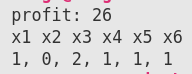
\includegraphics[]{9.png}
    \centering
    \caption{Результат работы программы}
\end{figure}